\chapter{Fotografias e Imagens dos Componentes}
\label{appendix:componentes}

Este anexo reúne as fotografias e imagens dos principais componentes utilizados no protótipo, referenciados ao longo do documento.

\section{Componentes Eletrónicos}

\begin{figure}[htbp]
  \centering
  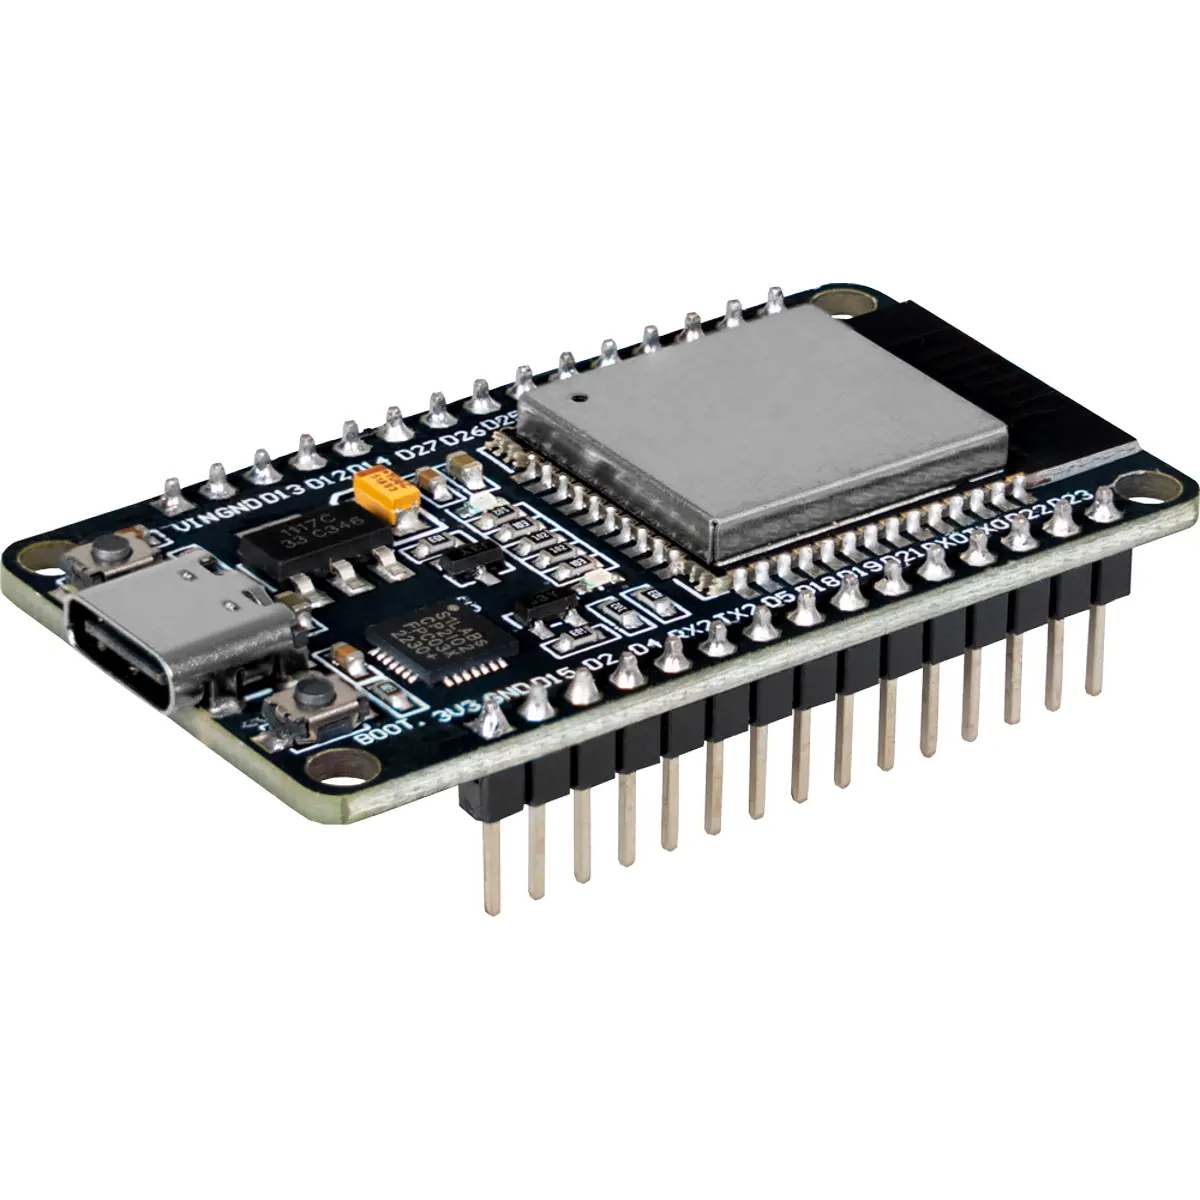
\includegraphics[width=0.45\textwidth]{figs/esp32.png}
  \caption{Módulo Joy-IT NodeMCU-ESP32-C utilizado como microcontrolador central~\cite{JoyITESP32}.}
  \label{fig:esp32-anexo}
\end{figure}

\begin{figure}[htbp]
  \centering
  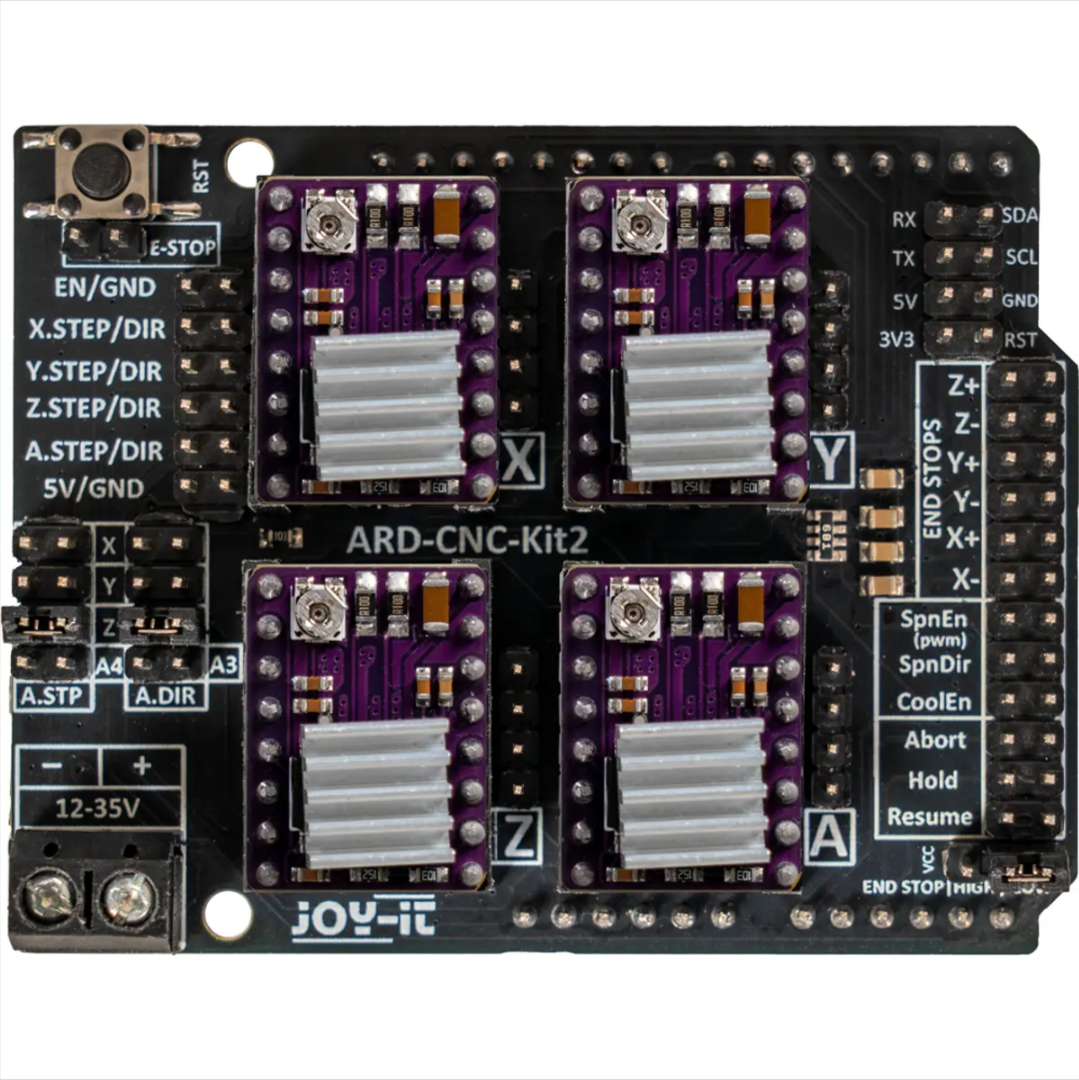
\includegraphics[width=0.65\textwidth]{figs/cnc_kit.png}
  \caption{Kit Joy-IT ARD-CNC-Kit2: CNC Shield com quatro módulos DRV8825 instalados~\cite{JoyITCNCKit2}.}
  \label{fig:cnc-shield-anexo}
\end{figure}

\begin{figure}[htbp]
  \centering
  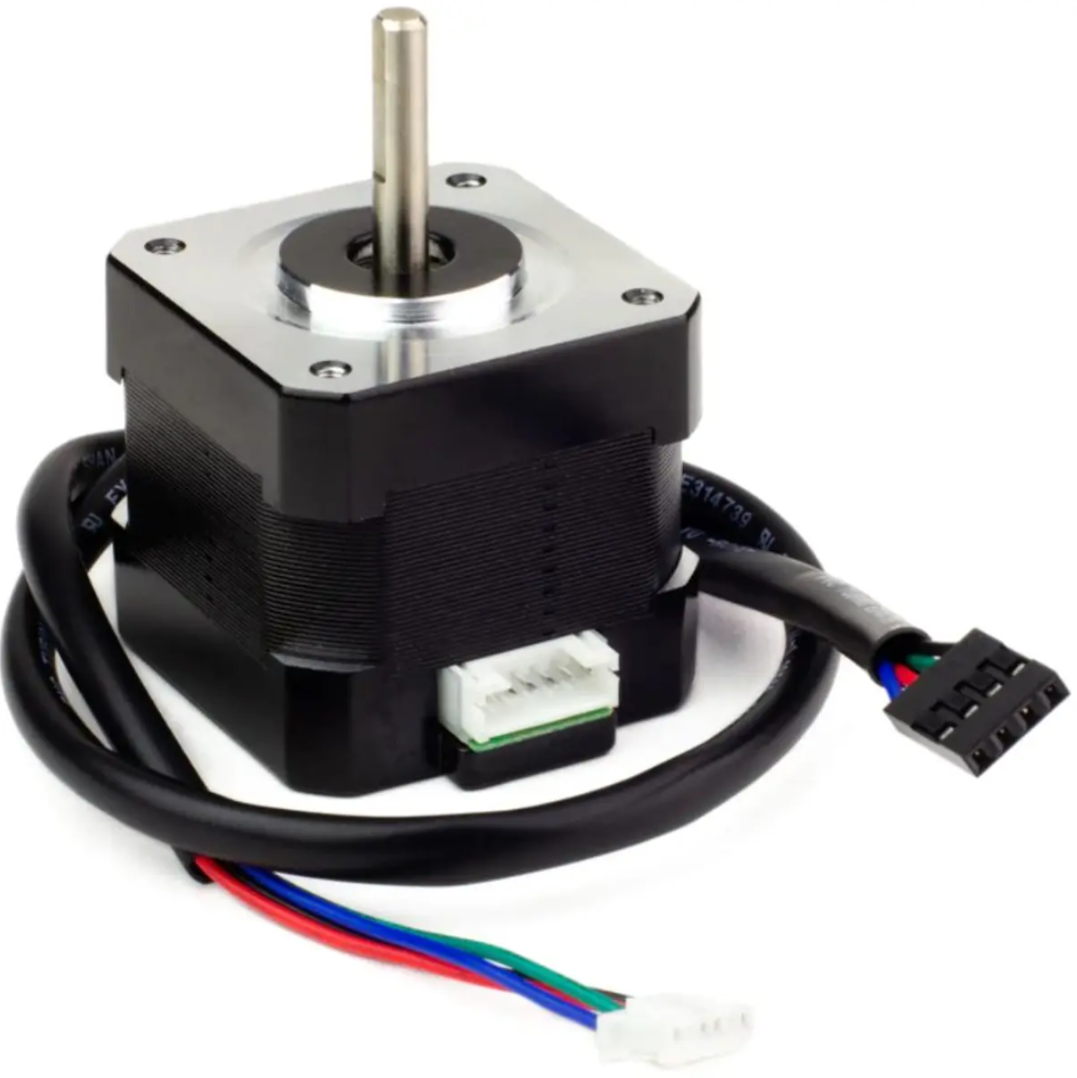
\includegraphics[width=0.45\textwidth]{figs/nema17.png}
  \caption{Motor de passo Joy-IT NEMA17-04~\cite{JoyITNEMA17}.}
  \label{fig:nema17-anexo}
\end{figure}

\begin{figure}[htbp]
  \centering
  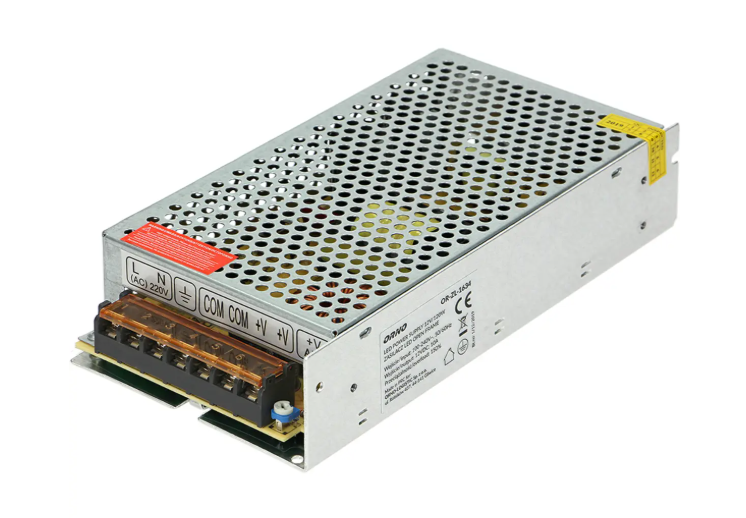
\includegraphics[width=0.6\textwidth]{figs/fonte_alimentacao.png}
  \caption{Fonte de alimentação DC ORNO OR-ZL-1636, 12\,V / 16,5\,A~\cite{FonteMauser}.}
  \label{fig:fonte-anexo}
\end{figure}

\section{Componentes Mecânicos}

\begin{figure}[htbp]
  \centering
  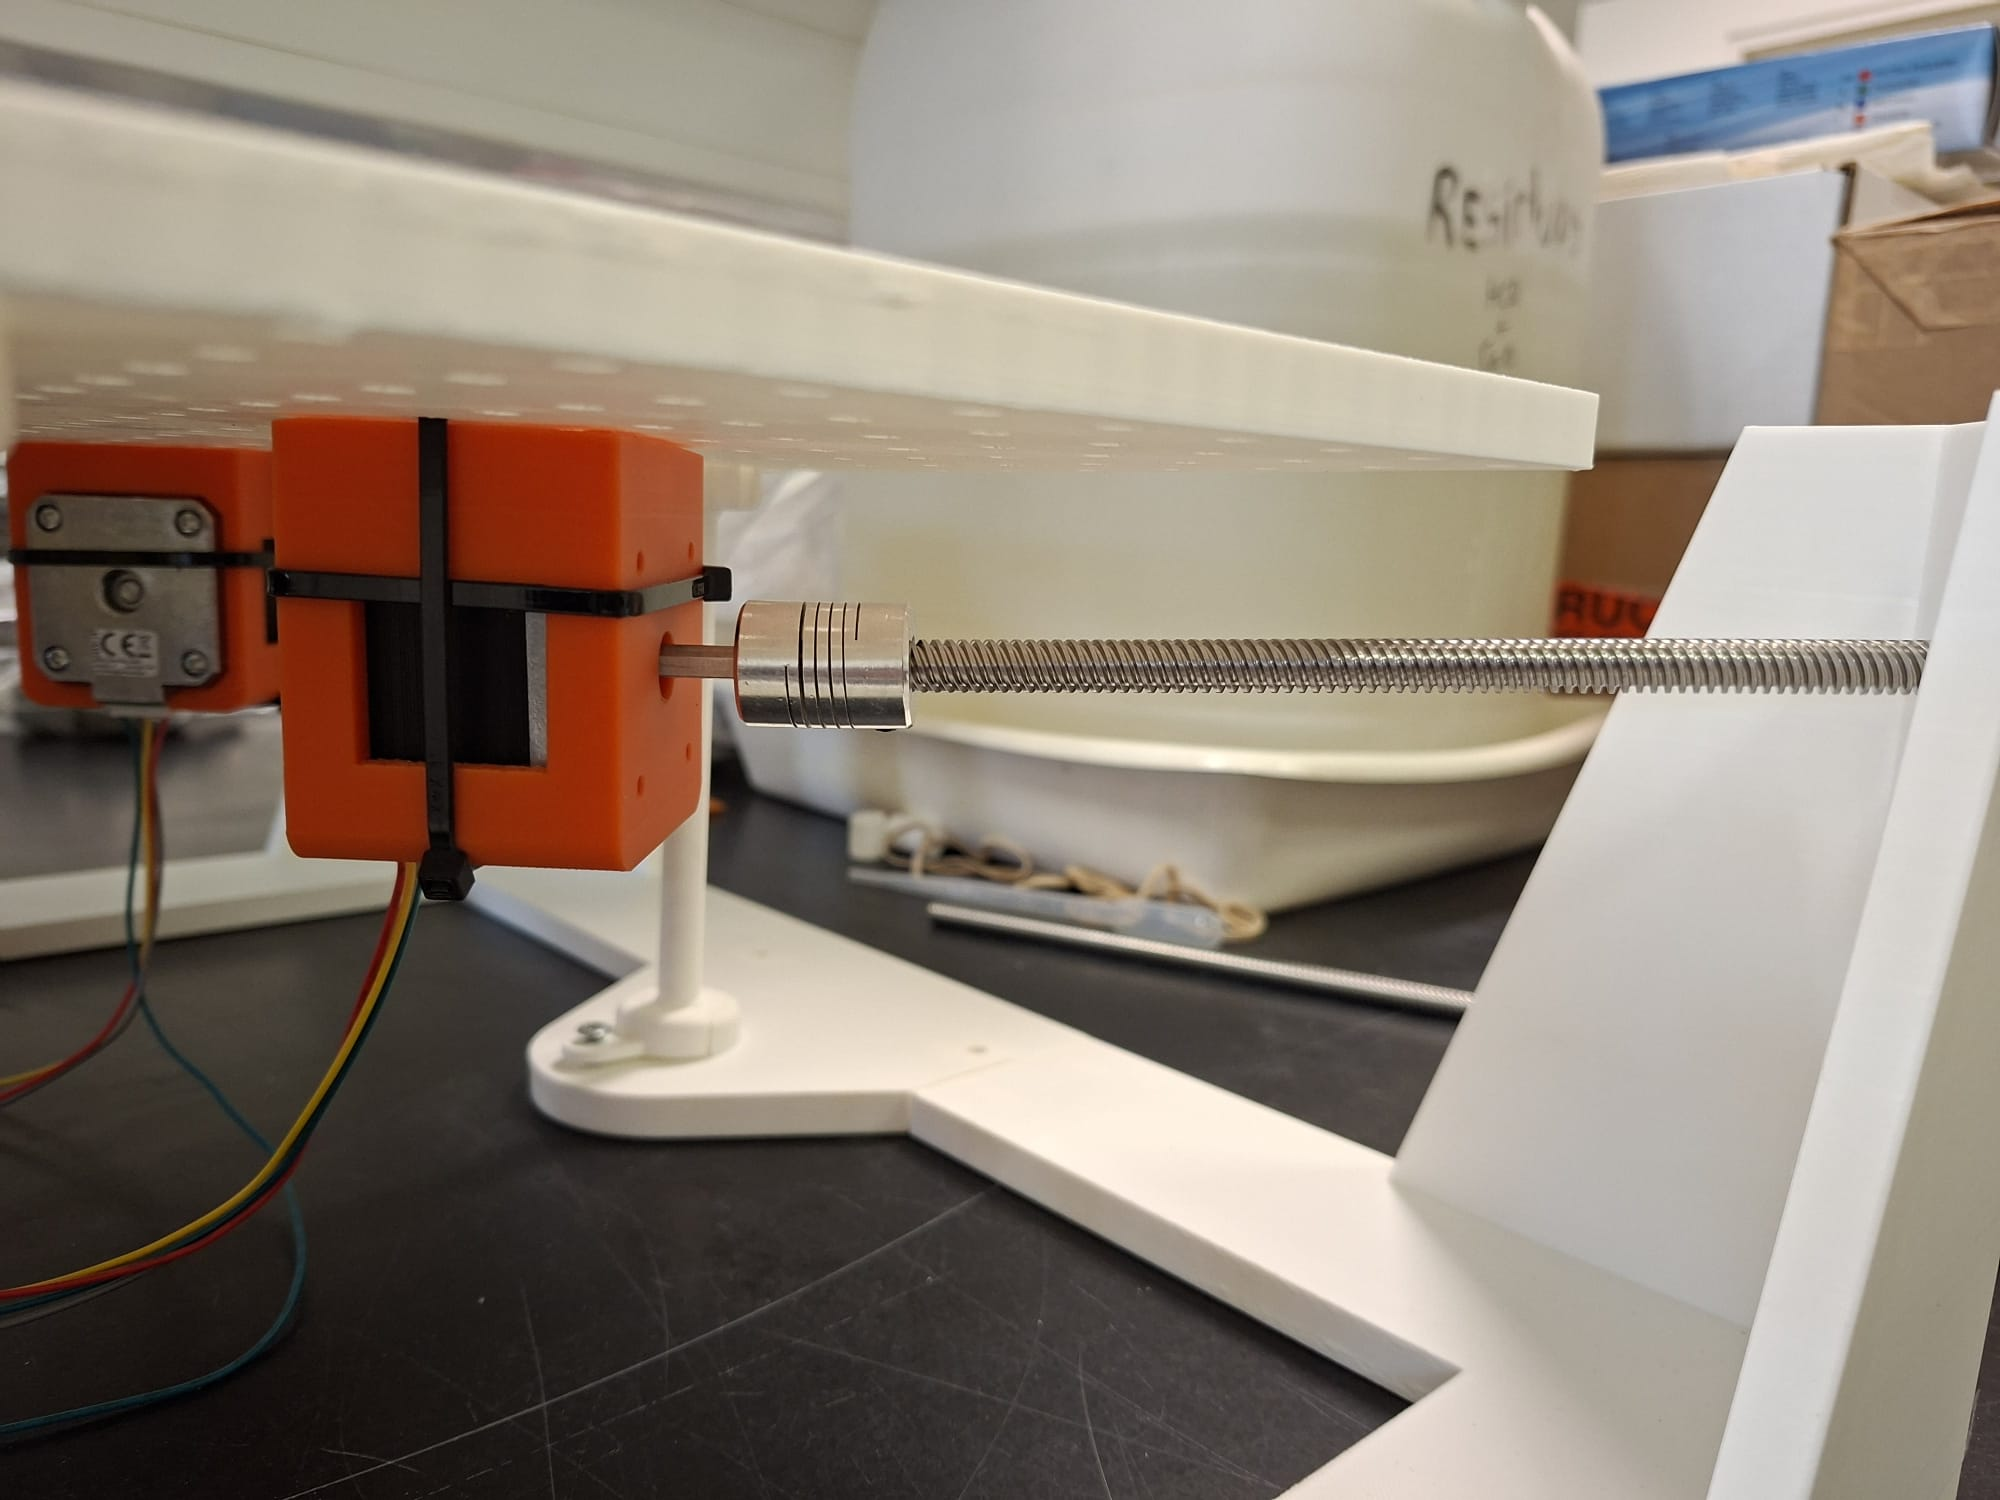
\includegraphics[width=0.6\textwidth]{figs/fuso_motor.jpeg}
  \caption{Acoplamento flexível motor-fuso~\cite{AcopladorAmazon}.}
  \label{fig:acoplador-anexo}
\end{figure}

\clearpage
\section{Protótipo Montado}

\begin{figure}[htbp]
    \centering
    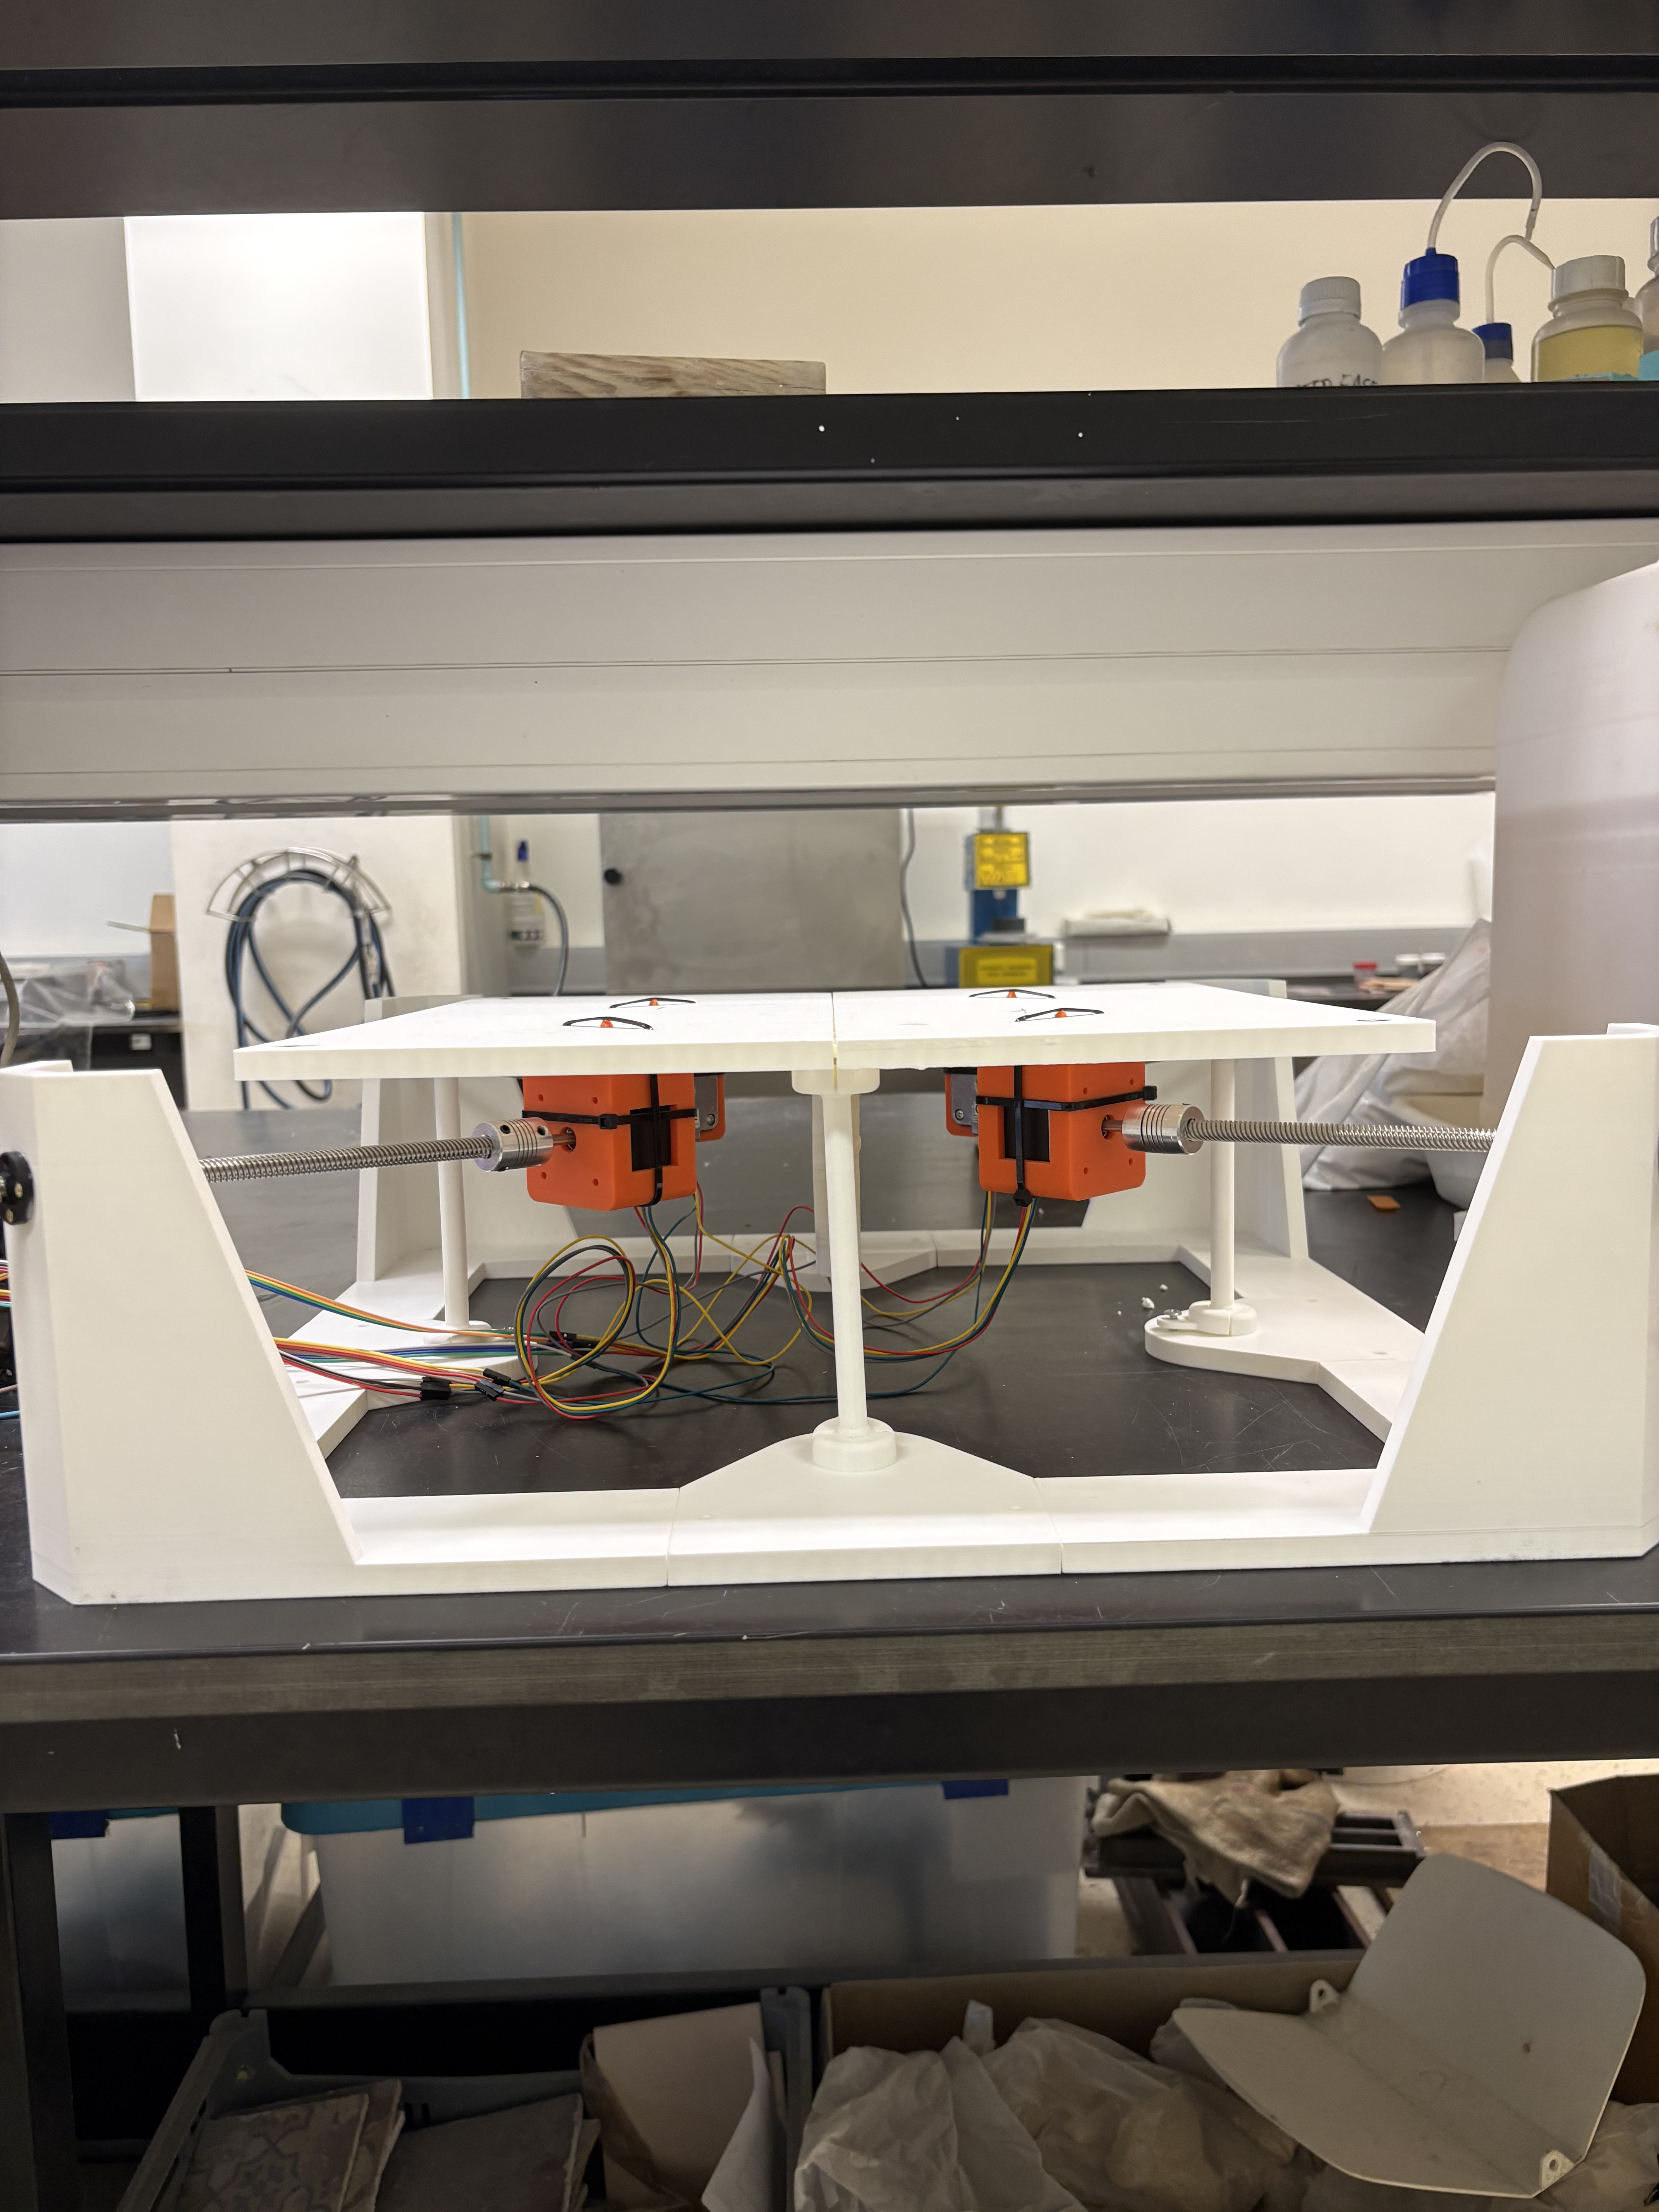
\includegraphics[width=0.75\textwidth]{figs/prototipo_frontal.png}
    \caption{Vista lateral do protótipo: plataforma móvel superior em PLA, quatro motores NEMA17 (laranja) com fusos TR8.}
    \label{fig:prototipo_lateral}
\end{figure}

\begin{figure}[htbp]
    \centering
    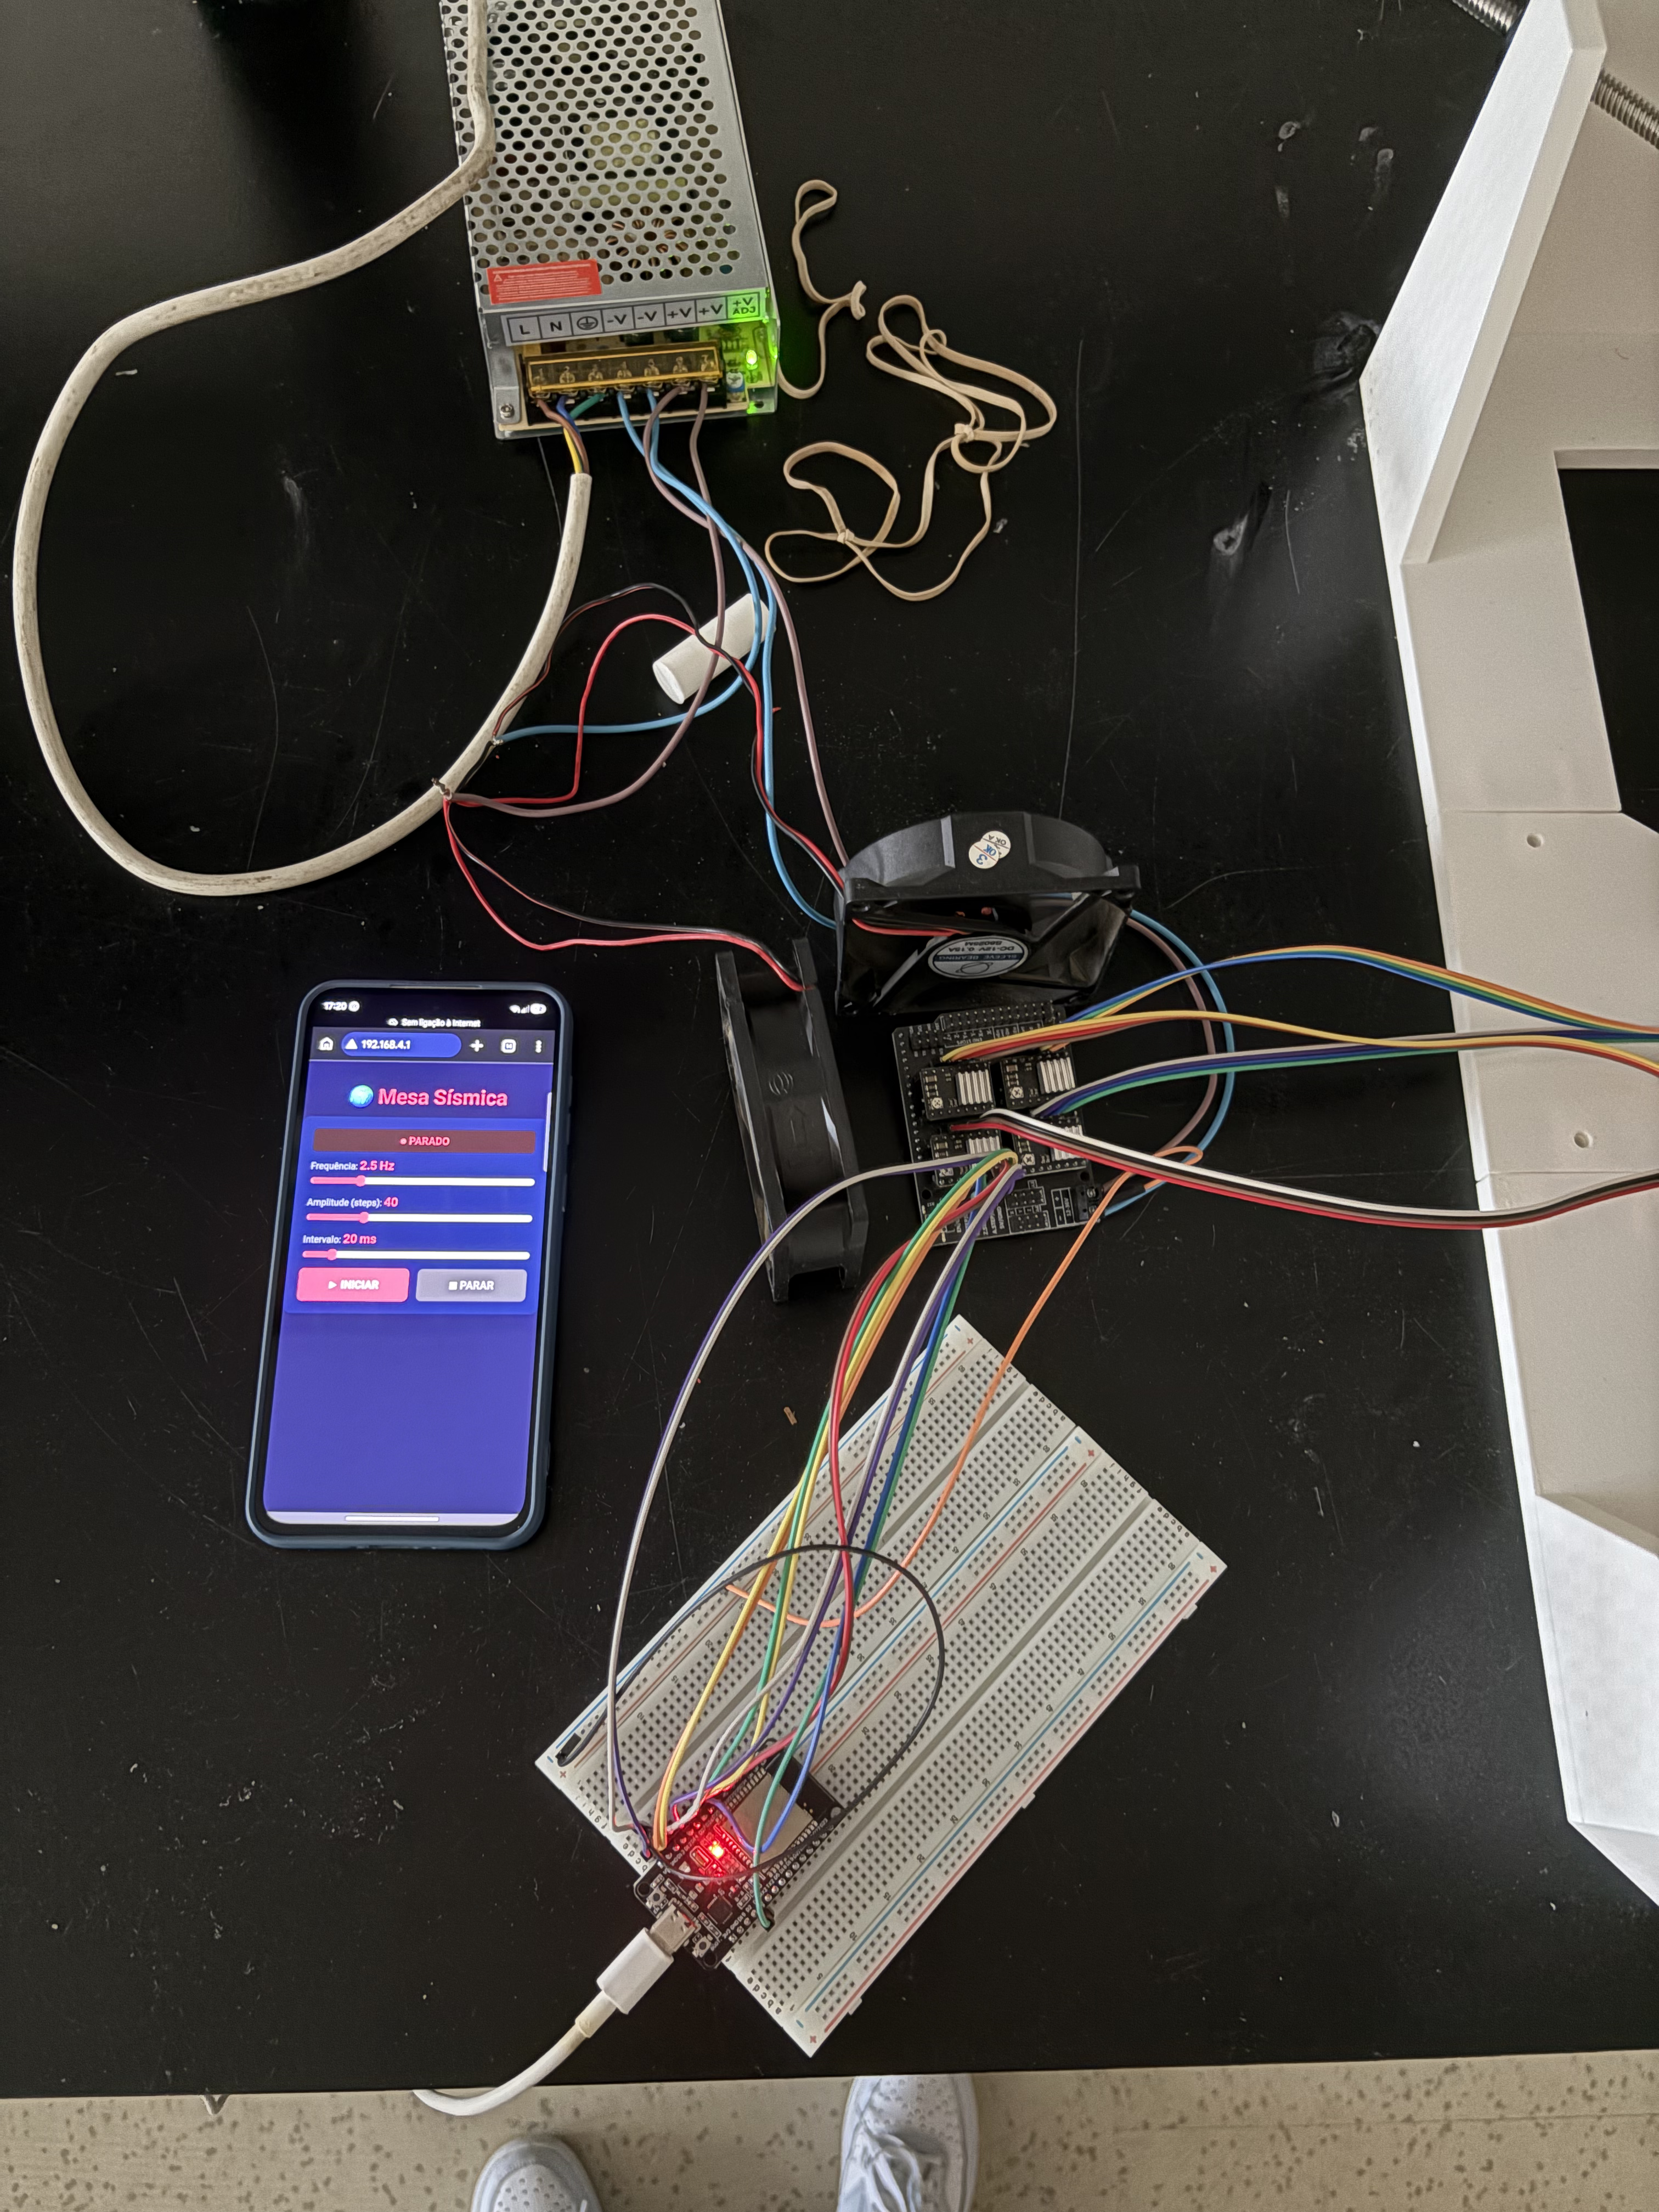
\includegraphics[width=0.75\textwidth]{figs/webui_smartphone.png}
    \caption{Interface web embarcada acedida via smartphone: a página servida pelo ESP32 em modo Access Point (\texttt{192.168.4.1}) permite configurar frequência, amplitude e intervalo, e iniciar ou parar o movimento sem ligação USB.}
    \label{fig:webui_smartphone}
\end{figure}

\begin{figure}[htbp]
    \centering
    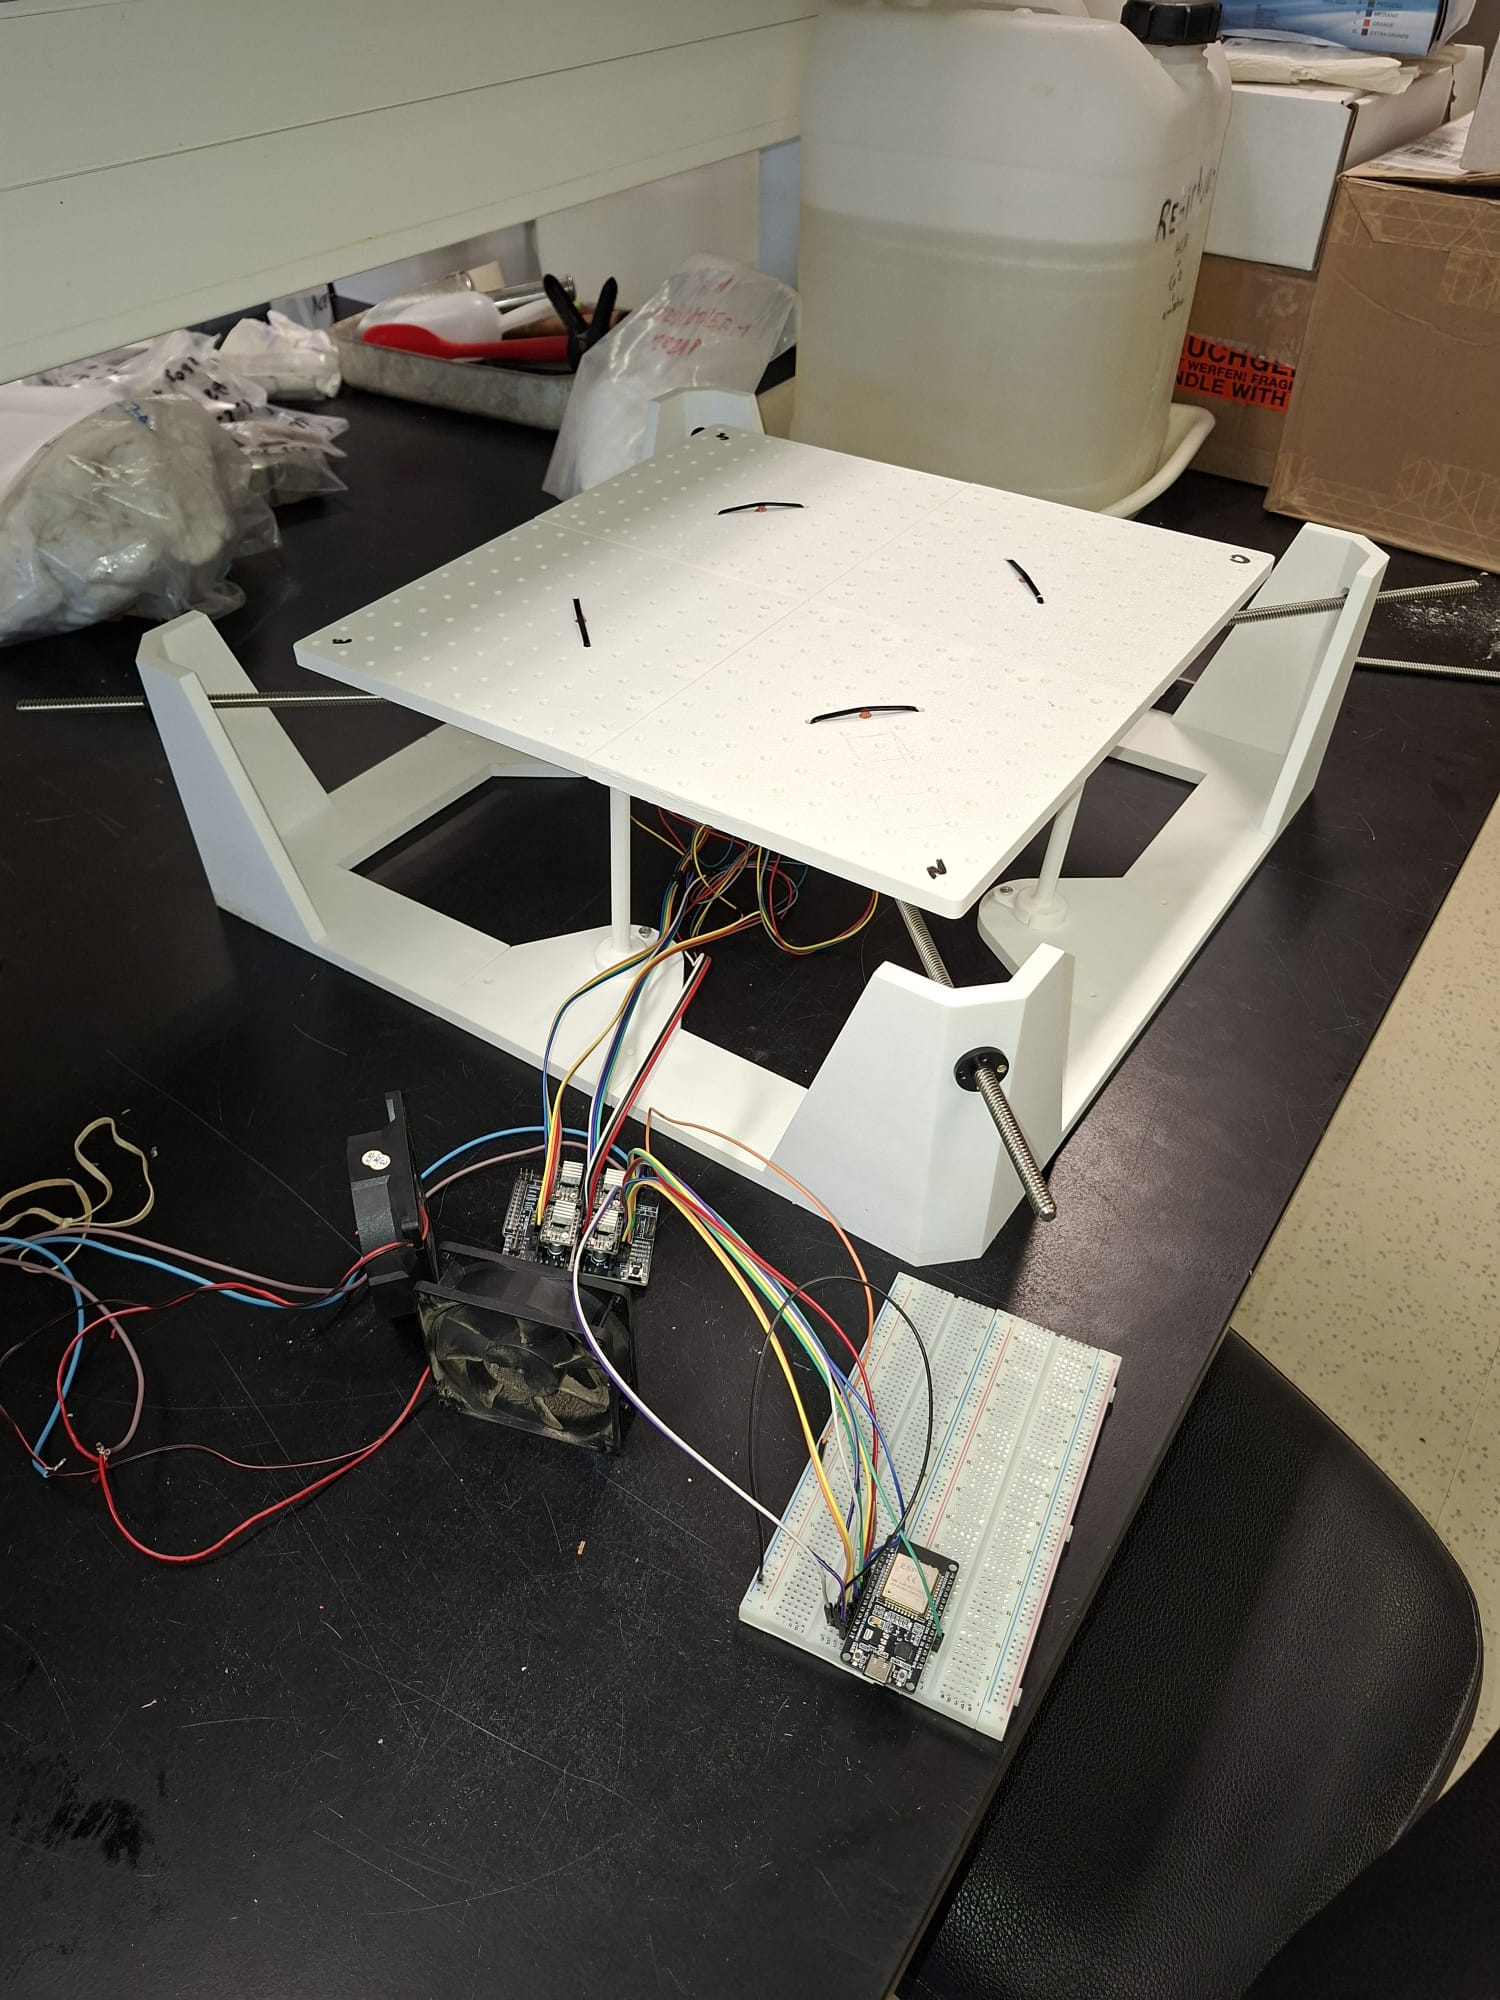
\includegraphics[width=0.75\textwidth]{figs/prototipo_lateral.jpeg}
    \caption{Vista frontal do protótipo: dois motores NEMA17 visíveis com fusos TR8, colunas de suporte em PLA e plataforma superior. A coluna central de apoio é visível ao centro da base.}
    \label{fig:prototipo_frontal}
\end{figure}

\begin{figure}[htbp]
    \centering
    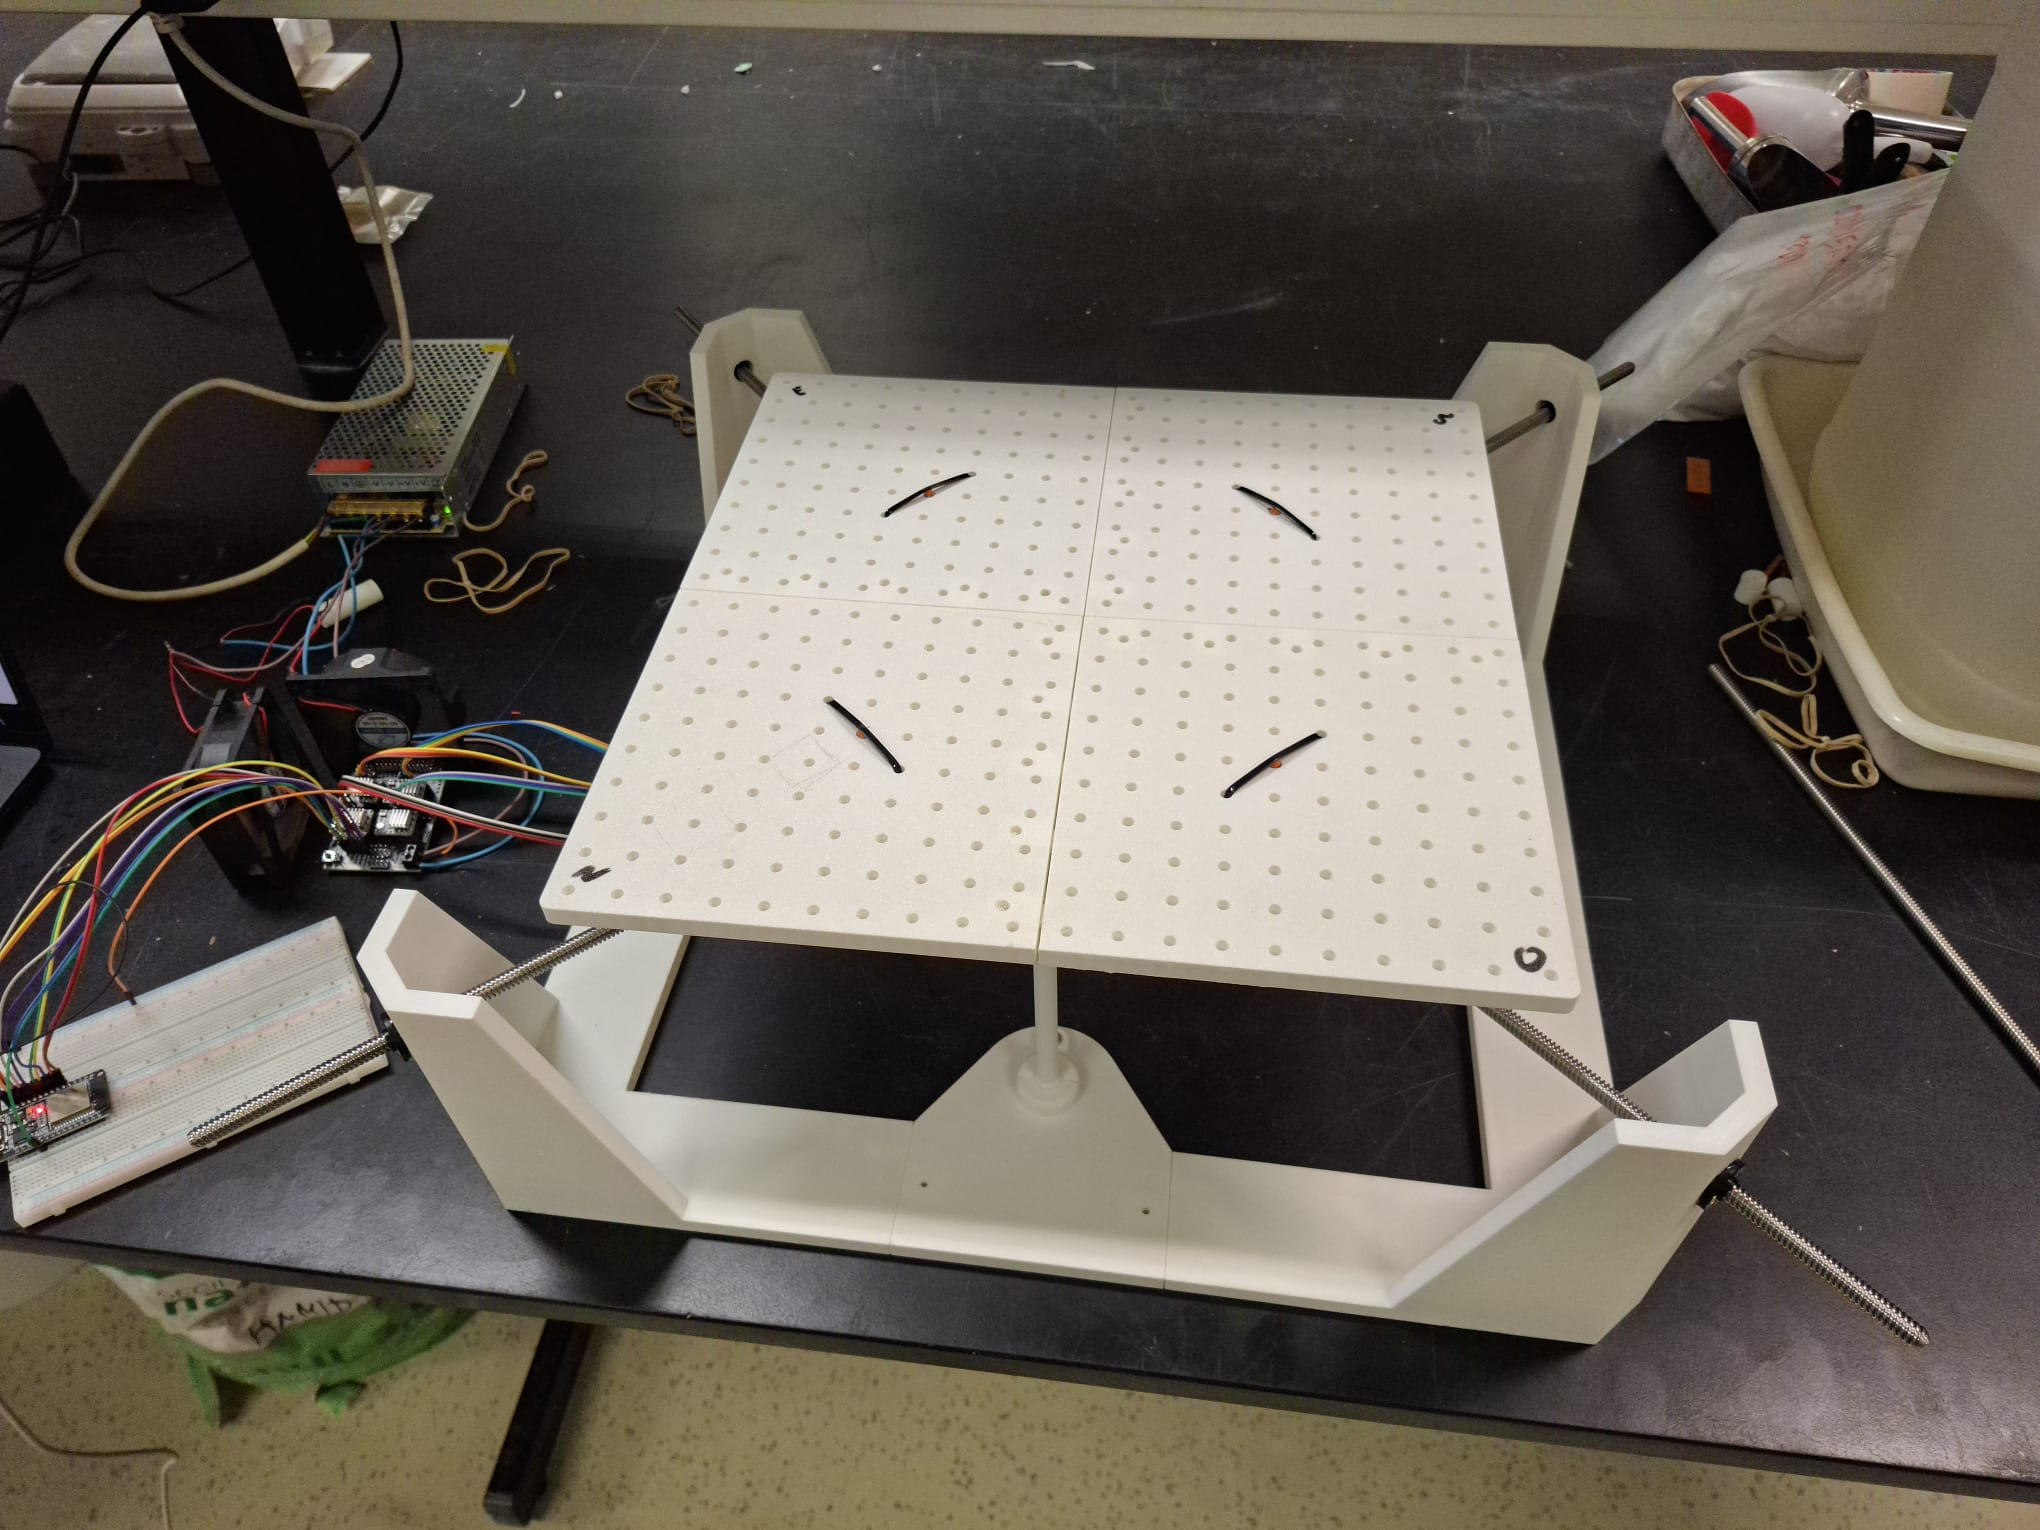
\includegraphics[width=0.75\textwidth]{figs/prototipo_topo.jpeg}
    \caption{Vista de topo do protótipo: plataforma superior dividida em quatro quadrantes com furo central de alinhamento e orifícios de fixação de modelos. As marcações N, S, E, W identificam a orientação de cada motor.}
    \label{fig:prototipo_topo}
\end{figure}